%\chapter{Desenvolvimento}
\label{desenvolvimento}
\section{Inserção Sequencial}
    Iniciando o desenvolvimento da prática, as arvores foram criadas na IDE assim como os vetores de tamanhos diversos para armazenar os valores que serão inseridos na arvore. Porém, o Java não permite a criação de vetores em 10\textsuperscript{9} elementos, então todas as arvores criadas, foram geradas até 10\textsuperscript{7} elementos. A partir disso, foi utilizada a função de inserção da classe arvore para inserir os elementos, mas como a inserção sequencial gastava muito tempo de execução, foi necessário criar uma função exclusiva de inserção para a arvore sequencial, o que reduziu bastante o tempo de execução, fazendo assim que fosse possível fazer a inserção sequencial em até 10\textsuperscript{7} elementos. Abaixo se tem uma comparação dos dois tipos de métodos para a inserção sequencial:\\
    Tempo de execução para inserção não otimizada:\\
    O tempo de execução de uma arvore com 10 elementos em milissegundos é: 1\\
    O tempo de execução de uma arvore com 1000 elementos em milissegundos é: 4\\
    O tempo de execução de uma arvore com 100000 elementos em milissegundos é: 11635\\
    O tempo de execução de uma arvore com 10000000 elementos em milissegundos é: 5184000000 (Tempo estimado)
    
        \begin{center}
            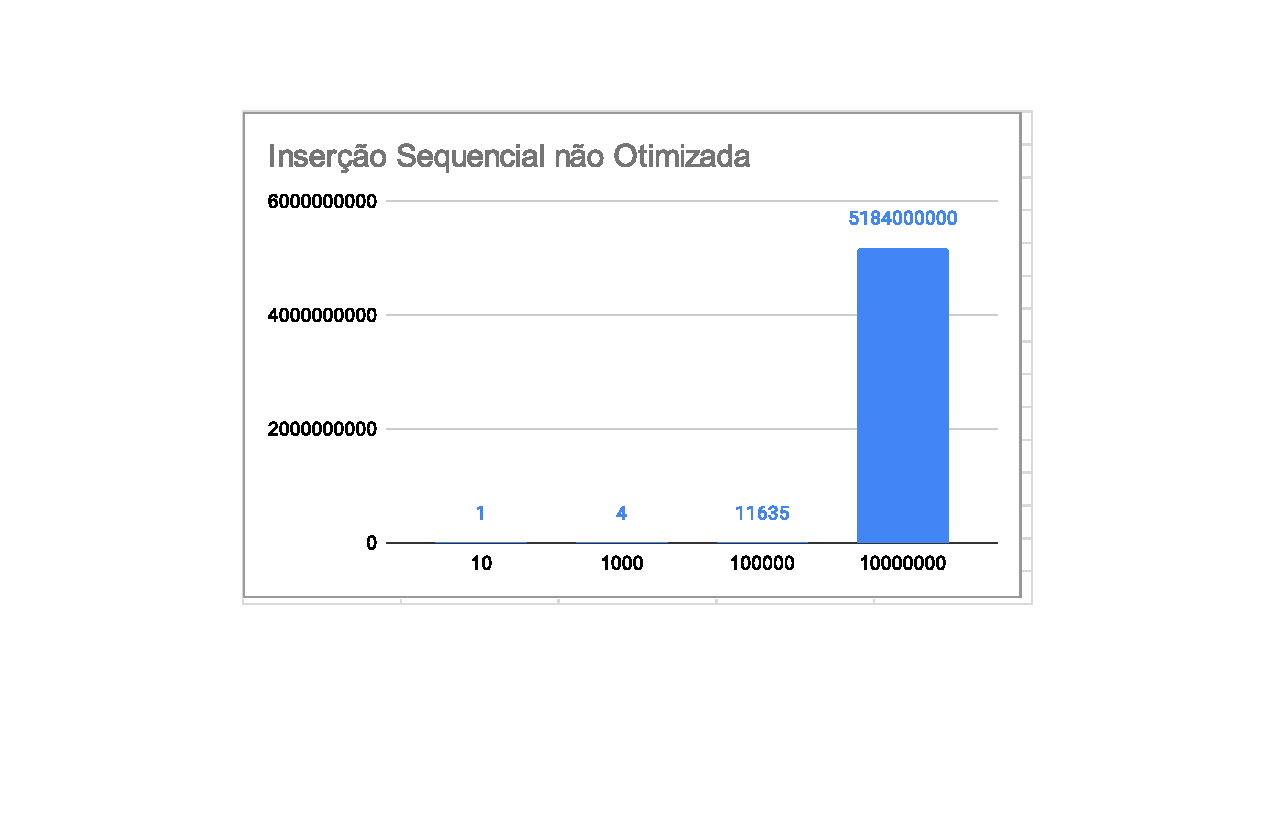
\includegraphics[scale=0.8]{Trabalho AED/fig/grafico1.pdf}
            \label{fig:Grafico 1}
        \end{center}
    Tempo de execução para inserção otimizada:\\
    O tempo de execução de uma arvore com 10 elementos em milissegundos é: 1\\
    O tempo de execução de uma arvore com 1000 elementos em milissegundos é: 1\\
    O tempo de execução de uma arvore com 100000 elementos em milissegundos é: 12\\
    O tempo de execução de uma arvore com 10000000 elementos em milissegundos é: 808\\
    
    \begin{center}
            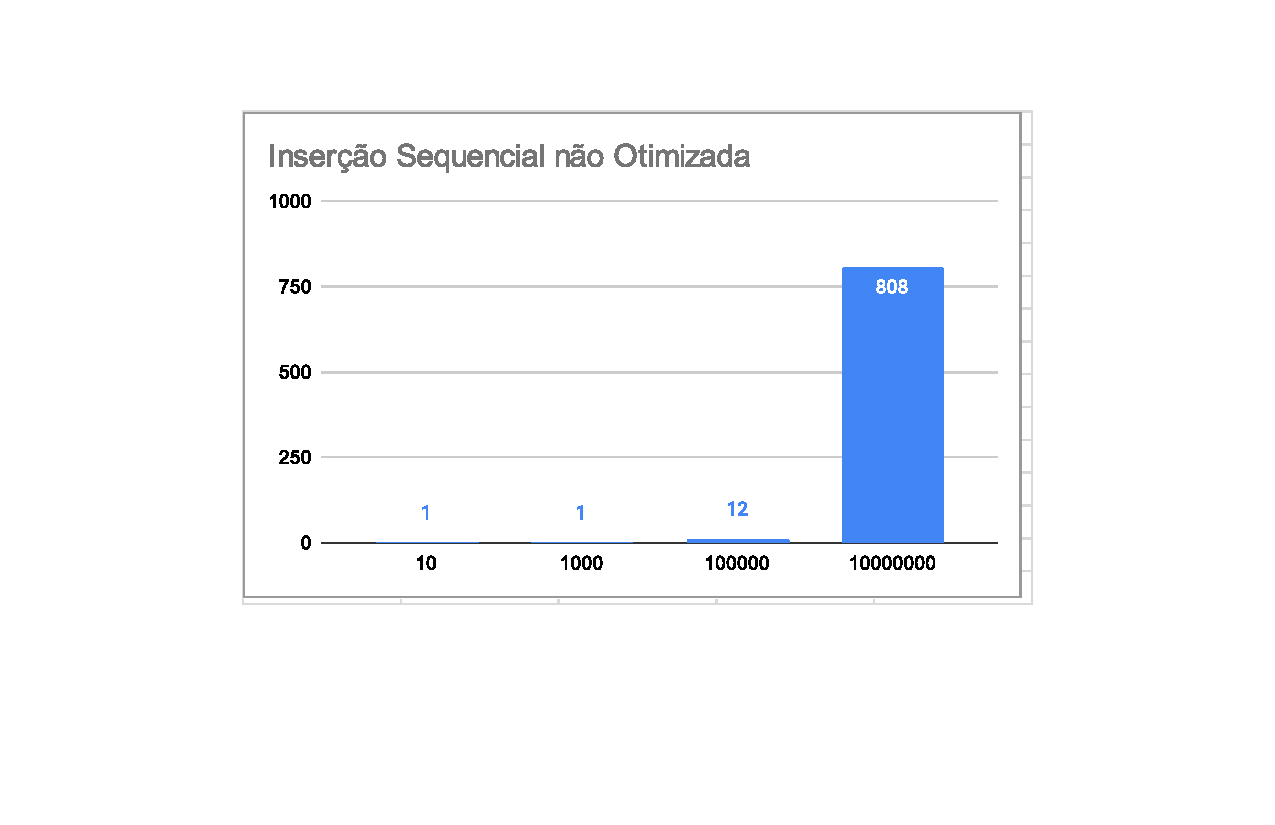
\includegraphics[scale=0.8]{Trabalho AED/fig/grafico2.pdf}
            \label{fig:Grafico 2}
    \end{center}
         \pagebreak
\section{Inserção Randômica}

Para a inserção randômica, foi utilizado o gerador congruencial linear, no qual foi utilizado os seguintes parâmetros:
        \begin{center}
        \\Semente = 0;
        \\Modulo = 1073741824;
        \\Multiplicador = 843314861;
        \\Incremento = 453816693;
        \end{center}
Dessa forma, utilizando a própria classe do gerador, um vetor era criado pra cada arvore, e assim que criado, era utilizado para inserir os valores na sua respectiva arvore, agora utilizando o método padrão de inserção da arvore, que dessa vez conseguia lidar com os valores e executar a tarefa completamente. Abaixo tem-se os tempos de execução para as inserções randômicas:\\
Tempo de execução para inserção randomizada:\\
O tempo de execução de uma arvore com 10 elementos em milissegundos é: 0\\
O tempo de execução de uma arvore com 1000 elementos em milissegundos é: 1\\
O tempo de execução de uma arvore com 100000 elementos em milissegundos é: 38\\
O tempo de execução de uma arvore com 10000000 elementos em milissegundos é: 11560
    \begin{center}
            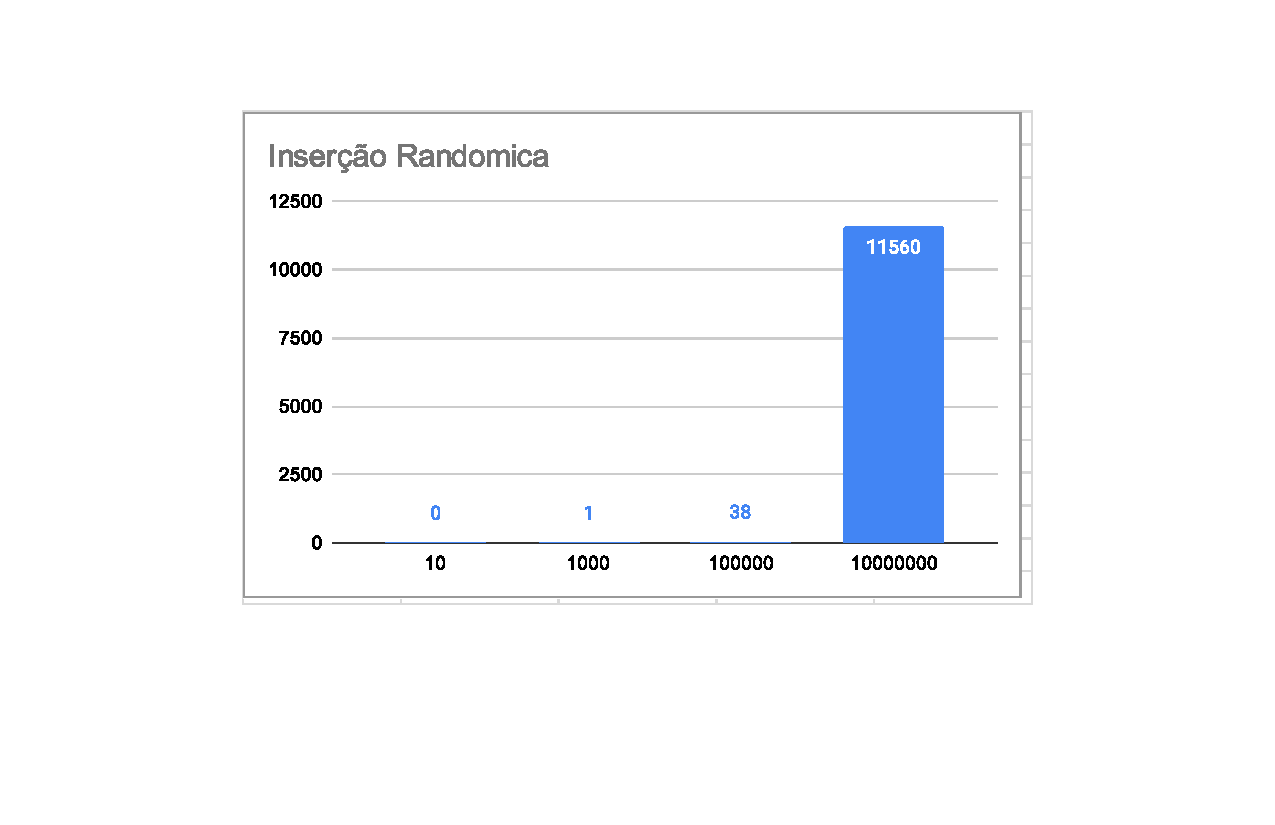
\includegraphics[scale=0.8]{Trabalho AED/fig/grafico3.pdf}
            \label{fig:Grafico 3}
    \end{center}
\pagebreak   
\section{Inserção Balanceada}

Para a inserção balanceada, foi necessário a criação de um método para que os valores fossem colocados de forma balanceada em um vetor. Assim que todos valores são inseridos de forma balanceada no vetor, o método de inserção na arvore é chamado, e então é utilizado o método de inserção padrão da arvore. Abaixo tem se os tempos de execução para a inserção na arvore balanceada:\\
Tempo de execução para inserção balanceada:\\
O tempo de execução de uma arvore com 10 elementos em milissegundos é: 0\\
O tempo de execução de uma arvore com 1000 elementos em milissegundos é: 0\\
O tempo de execução de uma arvore com 100000 elementos em milissegundos é: 6\\
O tempo de execução de uma arvore com 10000000 elementos em milissegundos é: 1472
    \begin{center}
            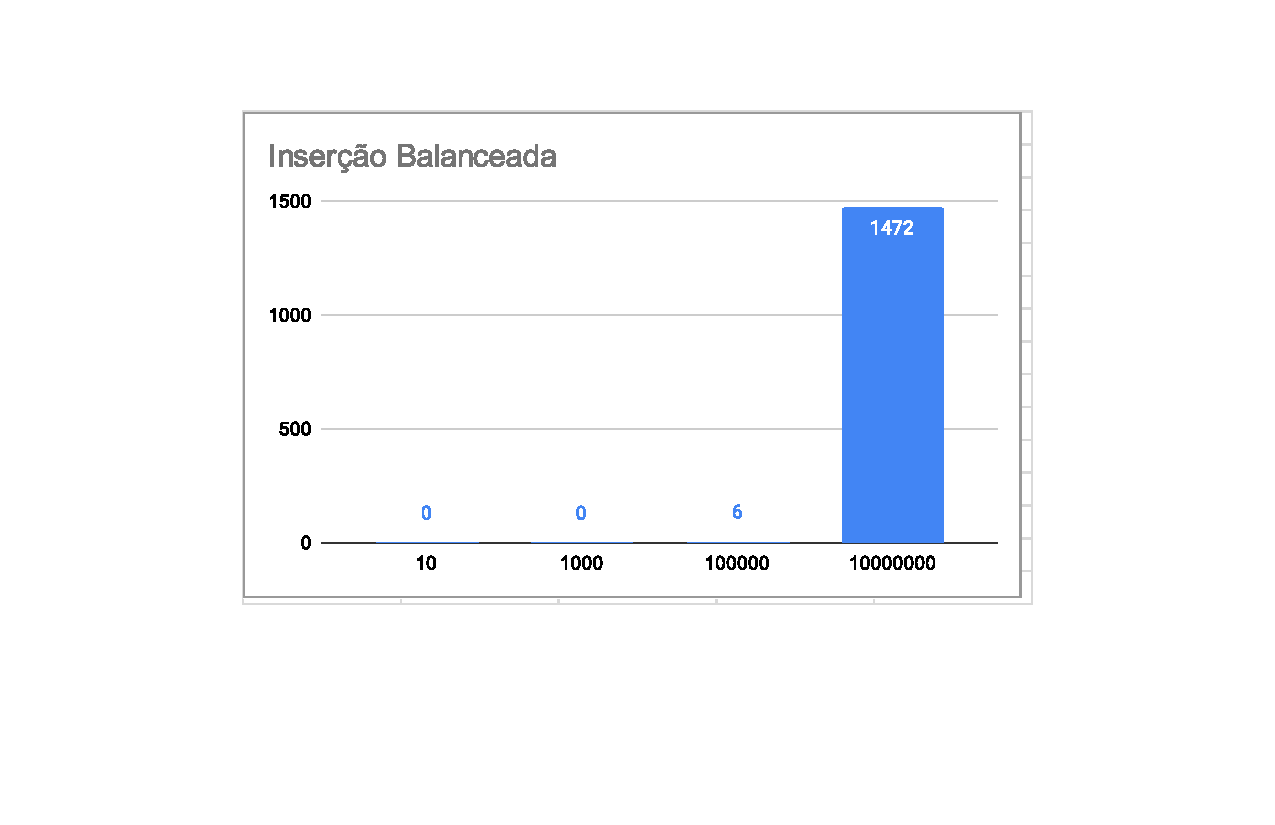
\includegraphics[scale=0.8]{Trabalho AED/fig/grafico4.pdf}
            \label{fig:Grafico 4}
    \end{center}
\pagebreak
\section{Busca}

Para fazer a média de 30 elementos na busca, foi utilizada o calculo em Nanosegundos, já que os valores em milissegundos seriam muito pequenos então dariam 0 em vários casos. Para cada arvore, foram feitas 30 buscas, e cada tempo de execução de cada busca era guardada como um elemento em um vetor de tamanho 30, para que depois fosse tirada a média. Essa média em breve será também utilizada para o calculo de Desvio Padrão. A formula da média seria:
        \begin{equation}
            Média = (\frac{X_{1}+X_{2}+X_{3}+...+X_{n}}{n}) 
        \end{equation}
No qual:
        \begin{center}
            \\O numerador é a soma dos termos numéricos
            \\O denominador é o total de termos;
        \end{center}

Abaixo tem os tempos de execução após o calculo de Média para cada arvore:
\\Média de busca na Arvore Sequencial\\
A media de busca da arvore 1 em nanosegundos foi de: 623\\
A media de busca da arvore 2 em nanosegundos foi de: 49586\\
A media de busca da arvore 3 em nanosegundos foi de: 527153\\
A media de busca da arvore 4 em nanosegundos foi de: 1569126
    \begin{center}
            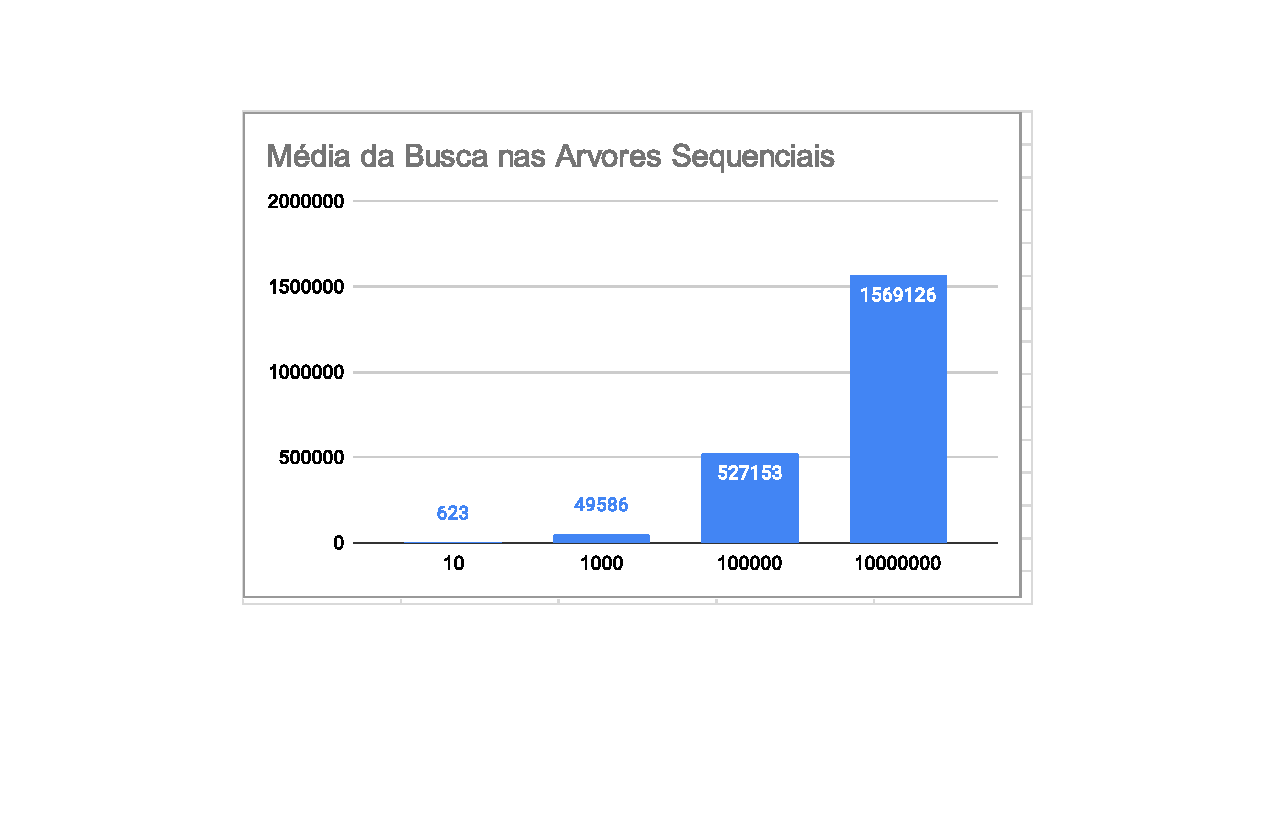
\includegraphics[scale=0.8]{Trabalho AED/fig/grafico5.pdf}
            \label{fig:Grafico 5}
    \end{center}
\pagebreak    
Média de busca na Arvore Randômica\\
A media de busca da arvore 5 em nanosegundos foi de: 4056\\
A media de busca da arvore 6 em nanosegundos foi de: 893\\
A media de busca da arvore 7 em nanosegundos foi de: 693\\
A media de busca da arvore 8 em nanosegundos foi de: 3850
    \begin{center}
            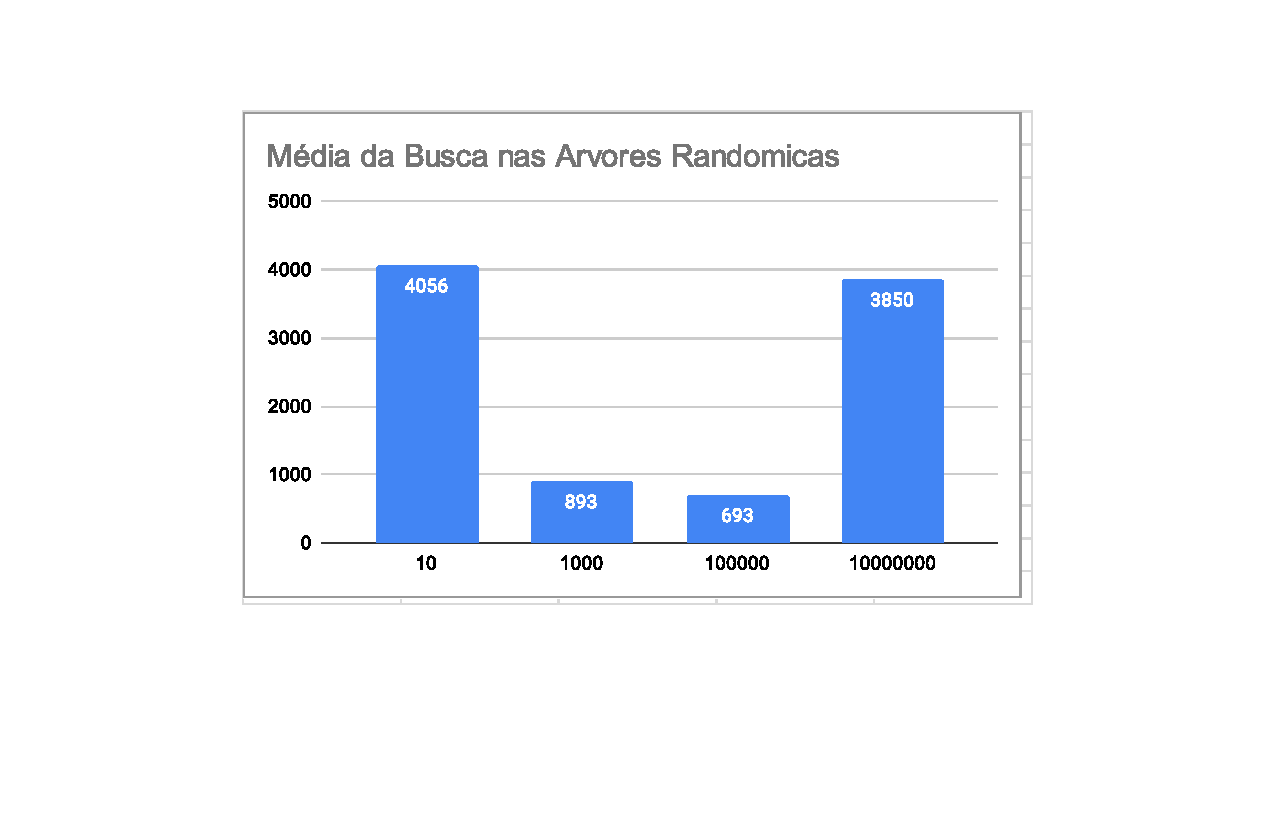
\includegraphics[scale=0.8]{Trabalho AED/fig/grafico6.pdf}
            \label{fig:Grafico 6}
    \end{center}
\pagebreak    
Média de busca na Arvore Balanceada\\
A media de busca da arvore 9 em nanosegundos foi de: 160\\
A media de busca da arvore 10 em nanosegundos foi de: 176\\
A media de busca da arvore 11 em nanosegundos foi de: 280\\
A media de busca da arvore 12 em nanosegundos foi de: 1150
    \begin{center}
            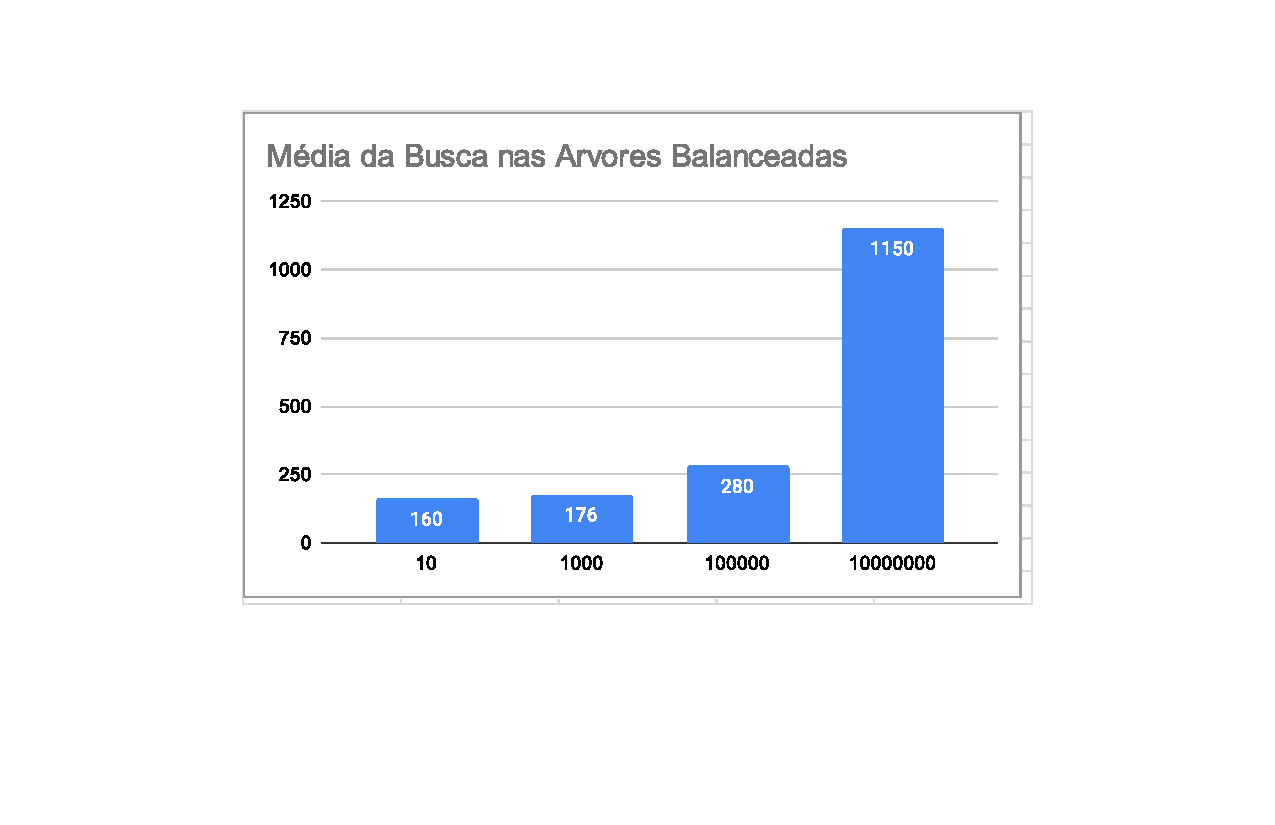
\includegraphics[scale=0.8]{Trabalho AED/fig/grafico7.pdf}
            \label{fig:Grafico 7}
    \end{center}
\pagebreak     
\section{Desvio Padrão}
Para calcular o Desvio Padrão da media dos tempos de busca da arvores, foi utilizado o vetor que armazenava cada um dos tempos de execução de busca de cada uma das arvores. A formula do desvio padrão consiste em:
    \begin{equation}
        s = \sqrt{\frac{\sum_{1}^N (x_i - m)^2}{N}}
    \end{equation}
            \begin{center}
            Onde é xi é valor na posição i no conjunto de dados\\
            m é a média\\
            N é a quantidade de dados\\
        \end{center}
Abaixo tem se os valores dos desvio padrão das arvores:\\
Desvio Padrão nas Arvores Sequenciais\\
O desvio padrão da arvore 1 em nanosegundos foi de: 628.056968399807\\
O desvio padrão da arvore 2 em nanosegundos foi de: 32571.600445104865\\
O desvio padrão da arvore 3 em nanosegundos foi de: 296333.56062983413\\
O desvio padrão da arvore 4 em nanosegundos foi de: 821931.0284493803
    \begin{center}
            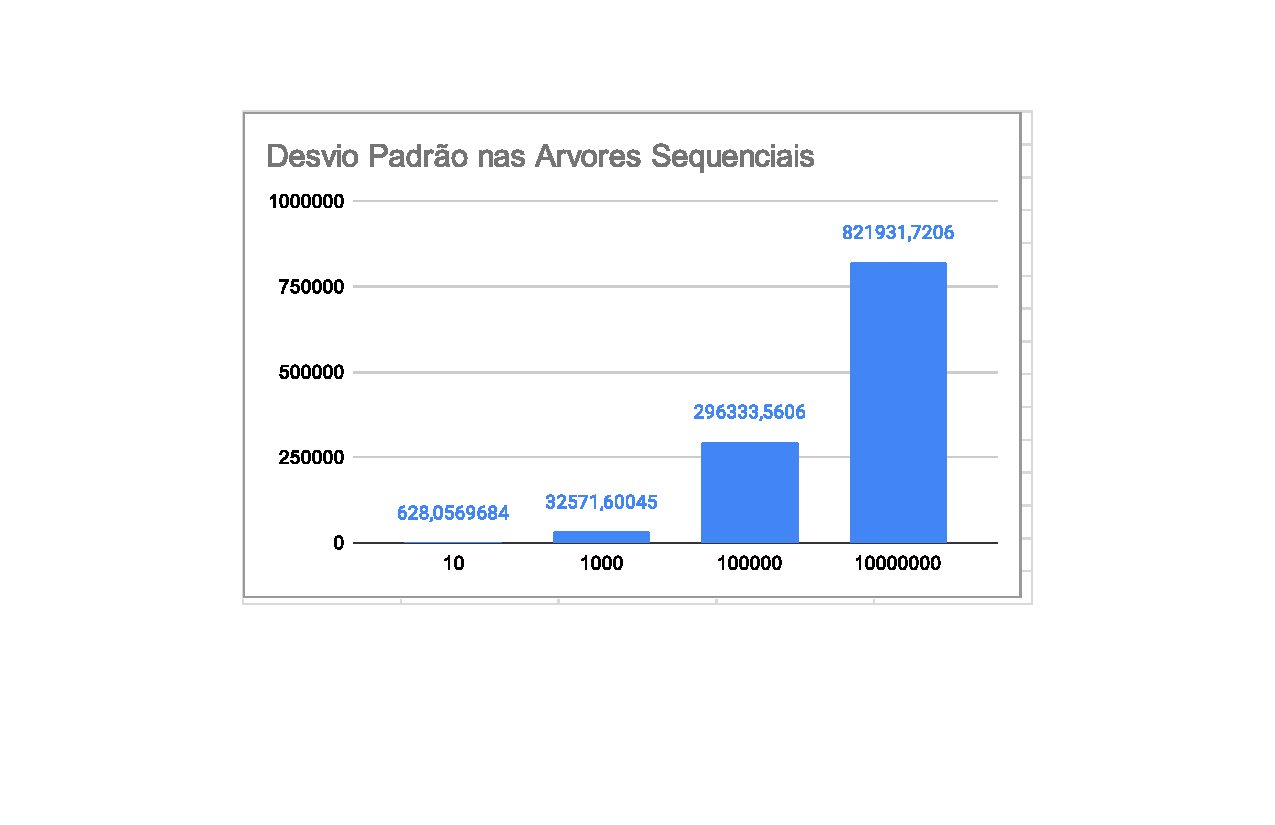
\includegraphics[scale=0.8]{Trabalho AED/fig/grafico8.pdf}
            \label{fig:Grafico 8}
    \end{center}
\pagebreak
Desvio Padrão nas Arvore Randômicas\\
O desvio padrão da arvore 5 em nanosegundos foi de: 14661.211485488573\\
O desvio padrão da arvore 6 em nanosegundos foi de: 444.17213880306457\\
O desvio padrão da arvore 7 em nanosegundos foi de: 463.99233710147496\\
O desvio padrão da arvore 8 em nanosegundos foi de: 14022.071886850388
    \begin{center}
            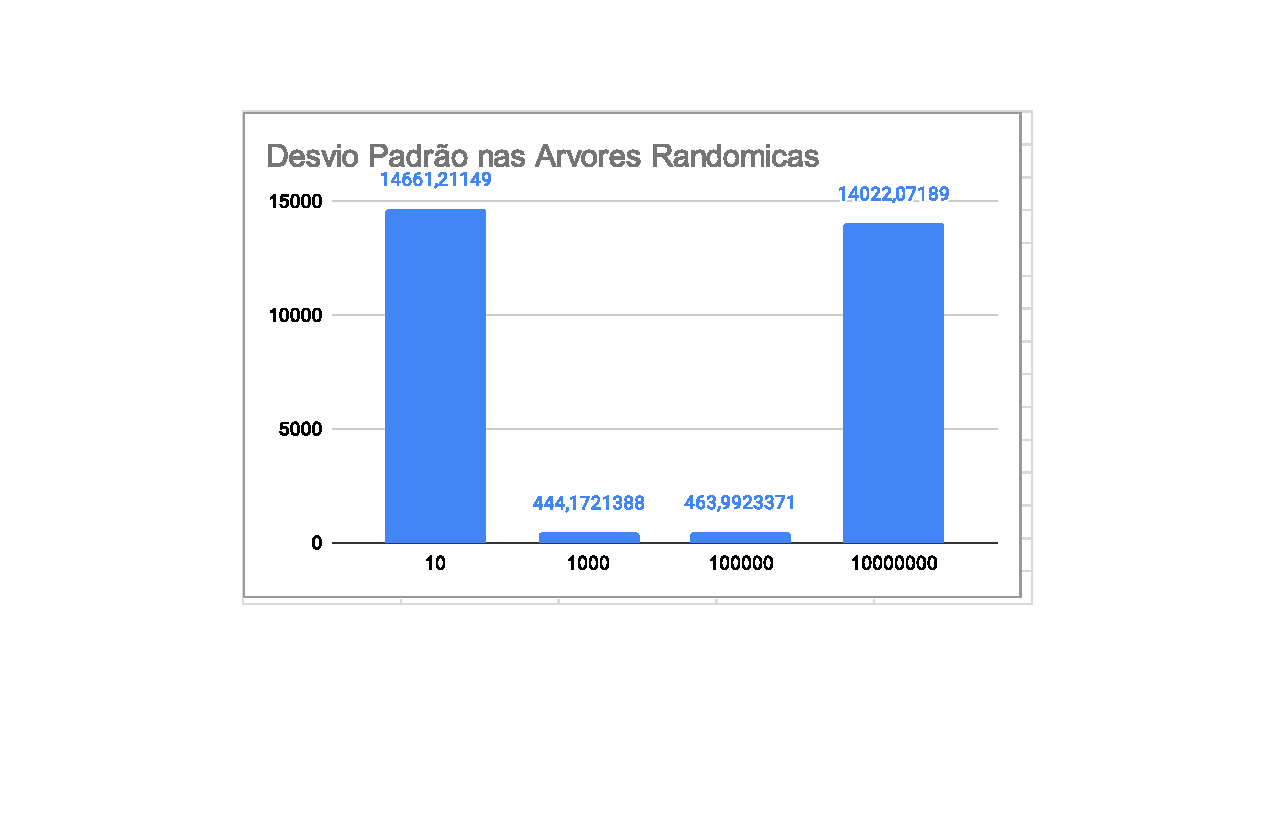
\includegraphics[scale=0.8]{Trabalho AED/fig/grafico9.pdf}
            \label{fig:Grafico 9}
    \end{center}
\pagebreak
Desvio Padrão nas Arvores Balanceadas\\
O desvio padrão da arvore 9 em nanosegundos foi de: 323.10988842807024\\
O desvio padrão da arvore 10 em nanosegundos foi de: 61.553951042064604\\
O desvio padrão da arvore 11 em nanosegundos foi de: 262.55158223353624\\
O desvio padrão da arvore 12 em nanosegundos foi de: 349.0463197533149
    \begin{center}
            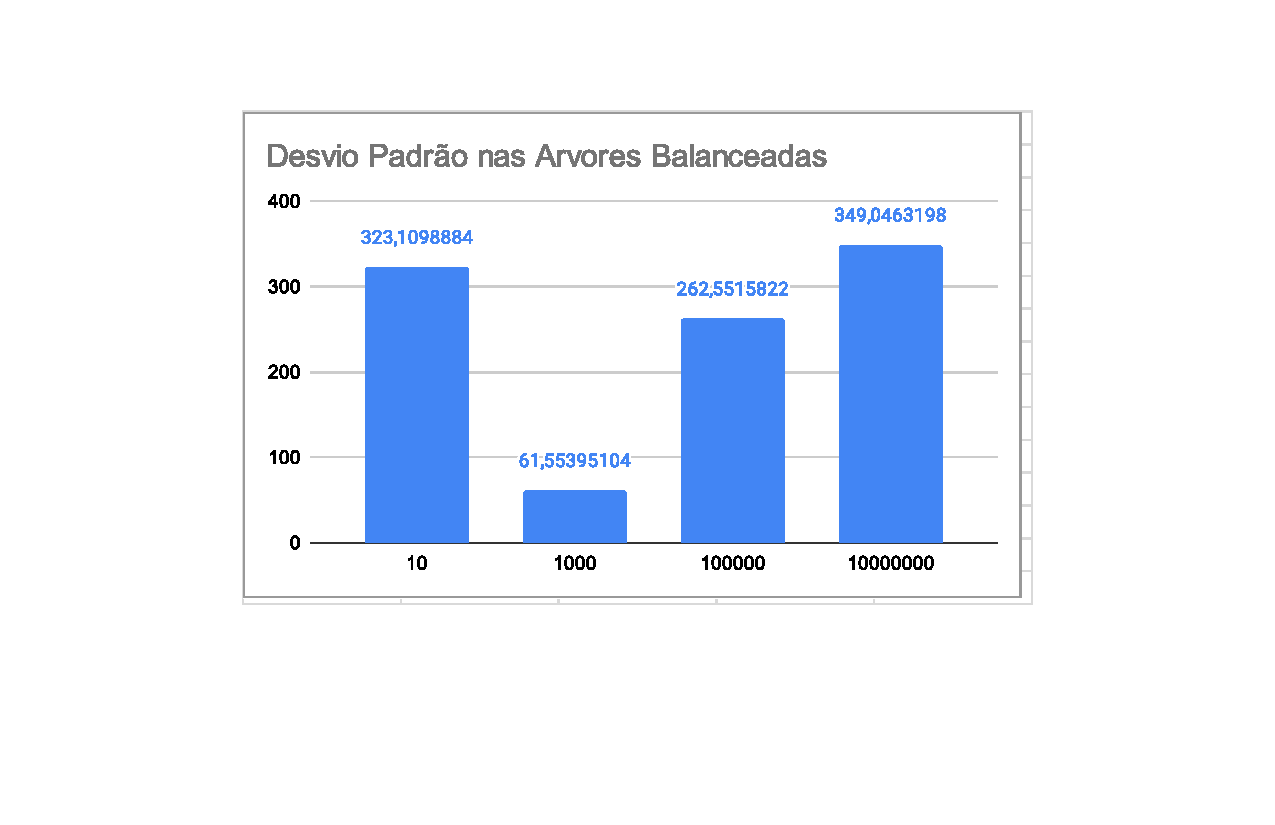
\includegraphics[scale=0.8]{Trabalho AED/fig/grafico10.pdf}
            \label{fig:Grafico 10}
    \end{center}